%Ne pas numéroter cette partie
\part*{Annexes}
%Rajouter la ligne "Annexes" dans le sommaire
\addcontentsline{toc}{part}{Annexes}

\section*{Annexe 1 - Raspberry Pi}
\addcontentsline{toc}{section}{Annexe 1 - Raspberry Pi}
    
    \begin{figure}[H]
        \centering
    	\begin{frame}{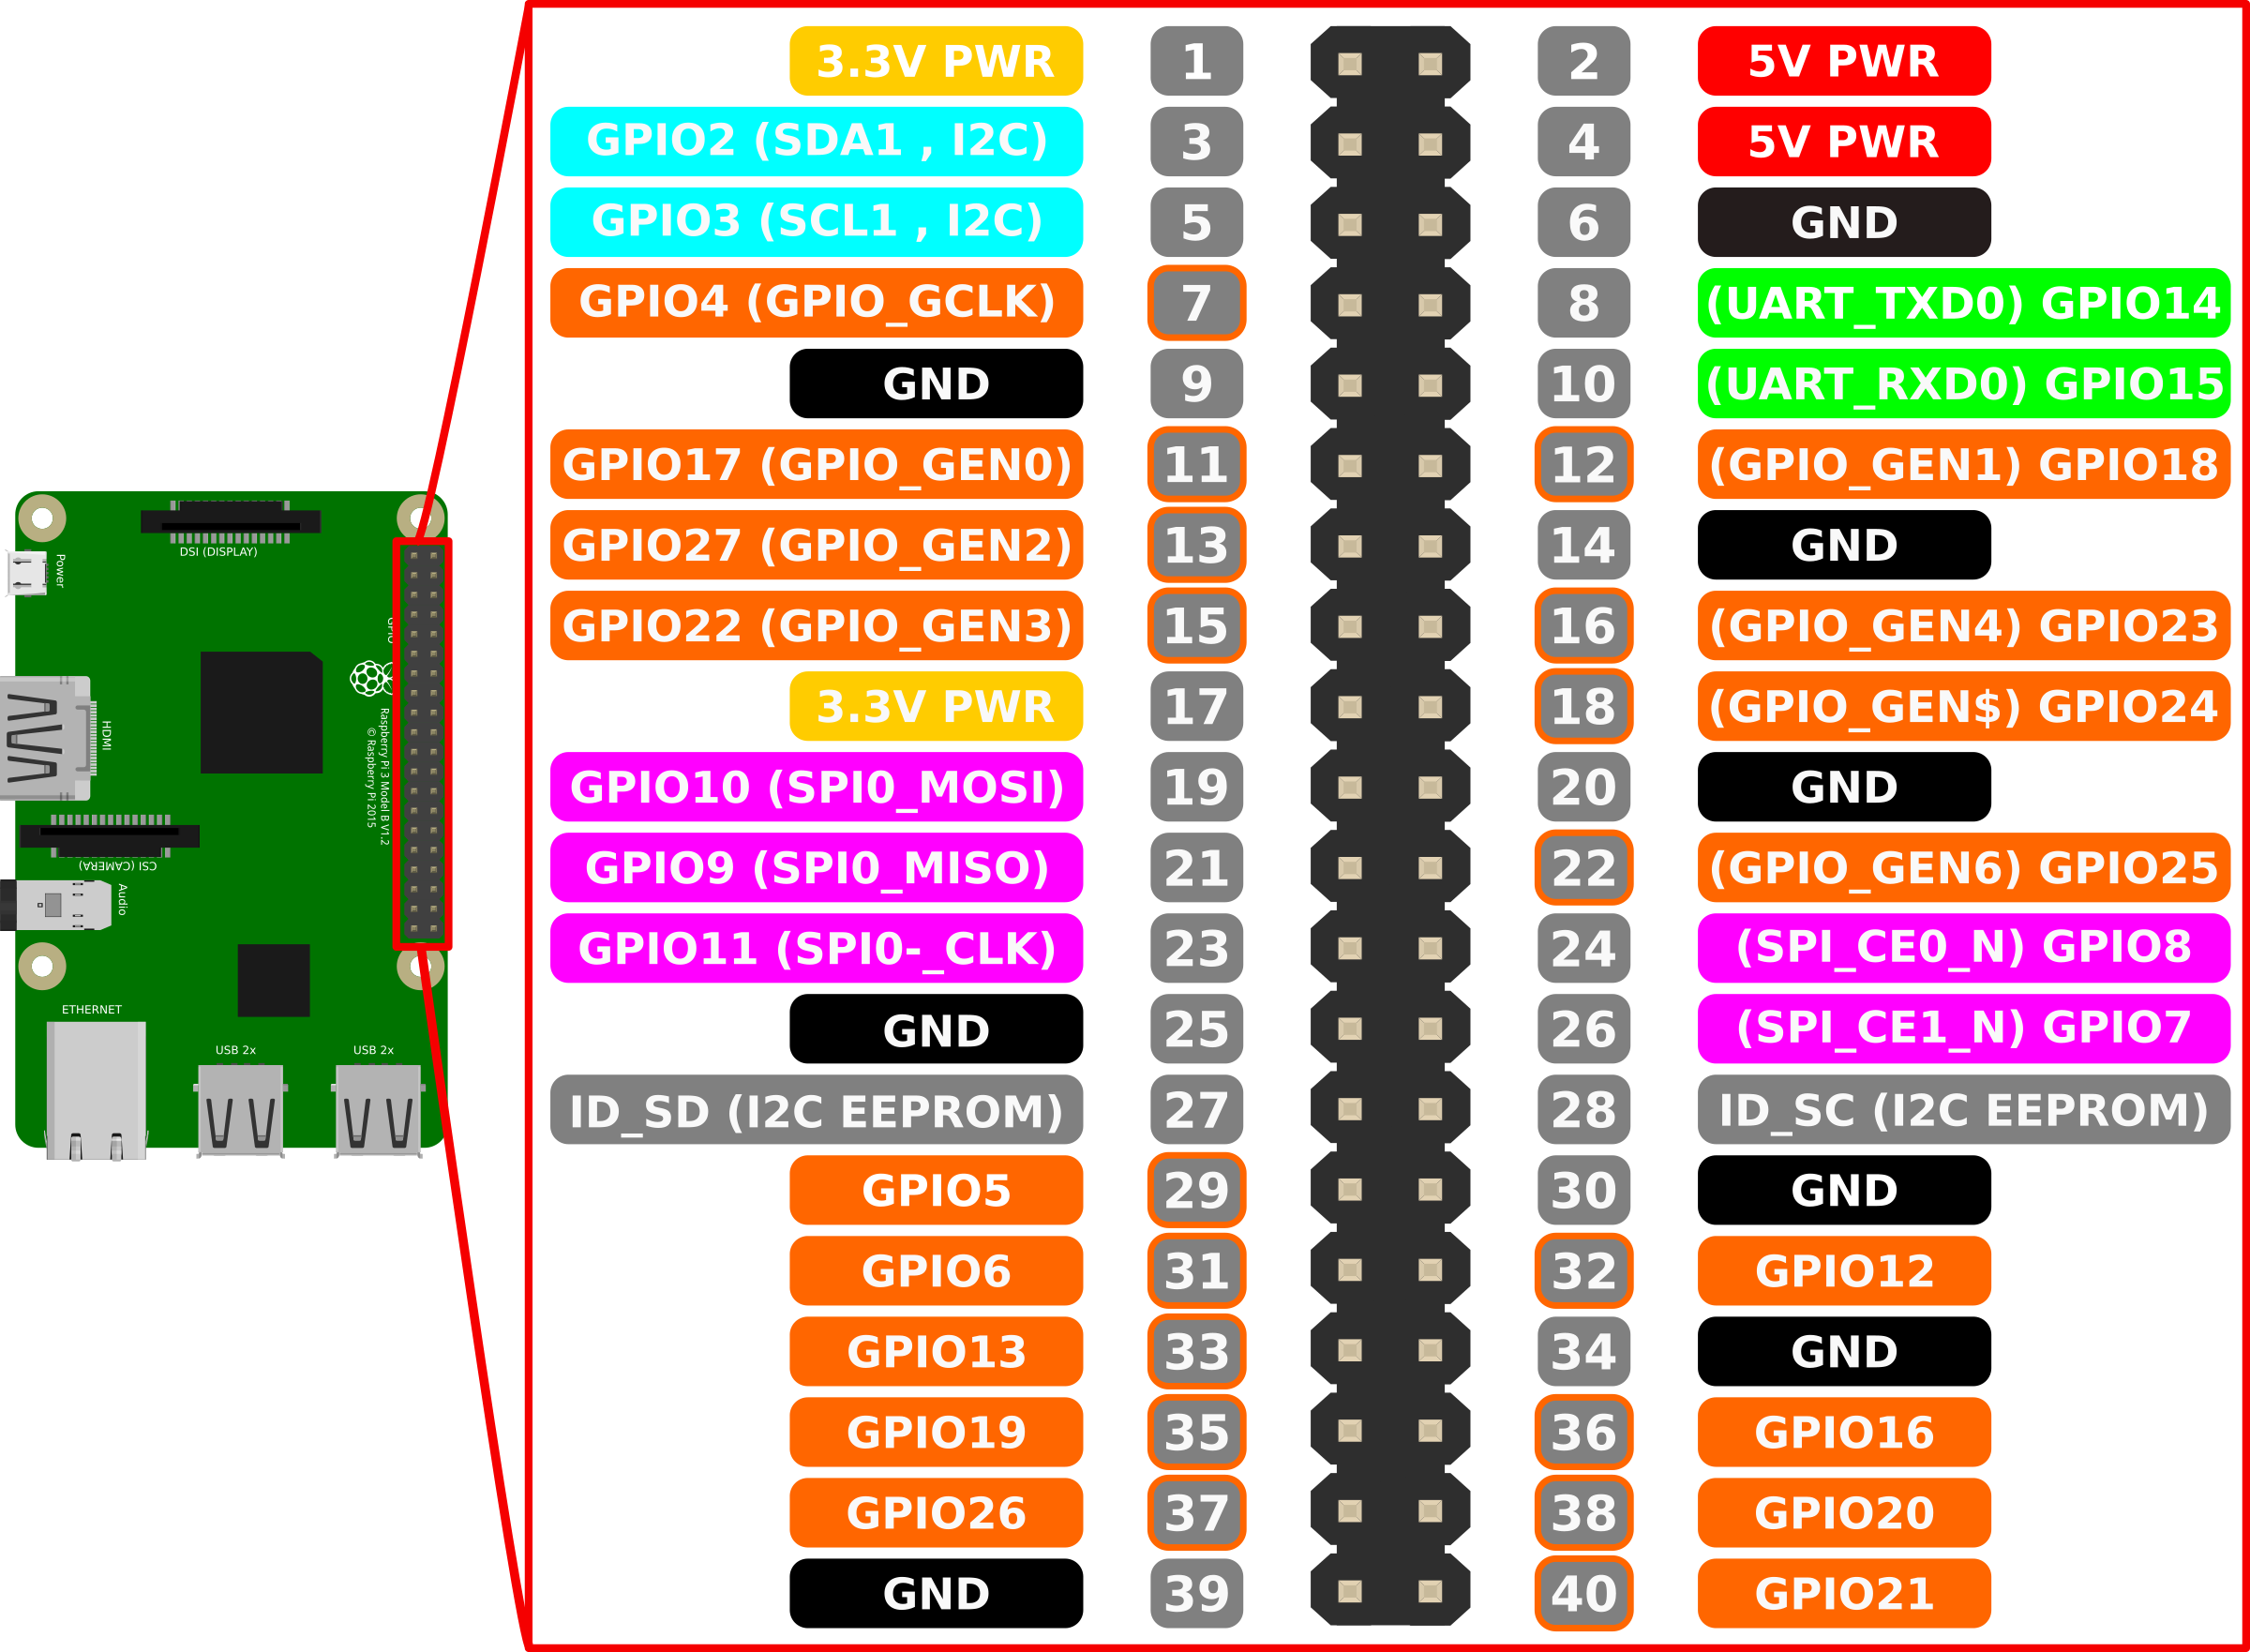
\includegraphics[width=1\textwidth]{image/gpioRPi.png}}
    	\end{frame}
    	\caption{\label{fig:gpioRPi}Détails des pins GPIO du Raspberry Pi 3 B+}
    \end{figure}
    
    \paragraph*{}
    Les pins qui m'ont été utiles étaient les pins 6 pour le GND, 8 et 10 pour le UART\_TX et UART\_RX.


\newpage
\section*{Annexe 2 - Code}
\addcontentsline{toc}{section}{Annexe 2 - Code}

    \paragraph*{}
    \lstinputlisting[caption={Connexion à l'automate}, label={code:connectServeur}]{"code/connexion.java"}
    
    \paragraph*{}
    \lstinputlisting[caption={Séparation des appels}, label={code:readVar}]{"code/readVar.java"}
    
    \paragraph*{}        
    \lstinputlisting[caption={Lecture des registres}, label={code:readAddr}]{"code/readAddr.java"}
    
    \paragraph*{}
    \lstinputlisting[caption={Exemple d'exécution sur un registre de type \%M}, label={code:execM}, language=TeX]{"code/execM.txt"}

    \paragraph*{}
    \lstinputlisting[caption={Exemple d'exécution sur un registre de type \%MW}, label={code:execMW}, language=TeX]{"code/execMW_noBDD.txt"}
    
    \paragraph*{}
    \lstinputlisting[caption={Fonction Java des requêtes SQL}, label={code:fctSQL}]{"code/fctSQL.java"}
    
    \paragraph*{}
    \lstinputlisting[caption={Exemple d'exécution sur un registre de type \%MW avec enregistrement dans la base de données}, label={code:execSQL}, language=TeX]{"code/execMW_bdd.txt"}
    
    \paragraph*{}
    
    
    \paragraph*{}
    
    
    \paragraph*{}
    
    
    \paragraph*{}
    
    